% 
% Information Retrieval
% -------------------------------
% University of California Irvine
% 
% Author:
% - María Carrasco Rodríguez
% - Fabs Lindenberg

\documentclass[a4paper,11pt,oneside]{book}
\usepackage{wrapfig} 
\usepackage{helvet}
\usepackage{phdthesis}
\usepackage{kostspielig}
\usepackage{amsmath}
\usepackage{multirow}
\usepackage{colortbl}
\usepackage{appendix}

\usepackage{color}
\usepackage{amsmath}
\usepackage{epsfig}


%\pagestyle{fancy}
%\fancyhead{}
%\fancyhead[L]{\textsf{\textbf{CS 221 Information Retrieval}\\ Assignment 2}}
%\fancyhead[R]{\textsf{Maria Carrasco (16874129)\\ Fabian Lindenberg (74076658)}}
%\fancyfoot[R]{\textsf{\thepage}}
%\renewcommand{\footrulewidth}{0.4pt}
%\cfoot[]{}


\newcommand{\todo}[1]{\textcolor{red}{\textbf{TODO: #1}}}

\hypersetup{colorlinks, 
           linkbordercolor= 1 0.8 0.8,
           citecolor=black,
           filecolor=black,
           linkcolor=black,
           urlcolor=black,
           bookmarksopen=true,
           pdftex}
\title{Information Retrieval }
\subtitle{Assignment 2}
\location{University of California Irvine}
\author{ María Carrasco Rodríguez (16874129) \\
		Fabian Lindenberg (74076658)}



\begin{document}

\kostspieligmaketitle

\tableofcontents
\pagebreak
% \startapendix

\chapter{General Questions}

\begin{enumerate}\item We issued the following ten queries:
				\begin{enumerate}
					\renewcommand{\labelenumii}{\Roman{enumii}}
					\item \texttt{google glasses}
					\item \texttt{google glasses news}
					\item \texttt{google glasses nytimes}
					\item \texttt{pidoco}
					\item \texttt{pidoco usability}
					\item \texttt{uci ics information retrieval winter 2011 assignment 2 christina lopes}
					\item \texttt{cordoba}
					\item \texttt{cordoba -argentina}
					\item $x^2 + 3x + 4 = 0$
					\item \texttt{sun}
				\end{enumerate}
				Formulating the first three queries, we tried to find the New York Times article\footnote{\url{http://www.nytimes.com/2010/11/28/business/28borker.html?pagewanted=all}} Professor Lopes talked about in class. Without specifying the name of the newspaper (first and second query), neither Google nor Bing listed the article on their first result page. After appending \texttt{nytimes} to the query string, both search engines ranked the article as the third result. In addition, a follow-up article was listed as the first (Bing) and fourth (Google) result, respectively.
				
				The fourth query searched for a specific start-up company based in Berlin, Germany. On Google, all results on the first page were closely related to that company (website, Wikipedia article, Facebook page, Twitter account, magazine articles, etc.). Bing, on the other hand, listed only the company website and the Wikipedia article; all other results of the first page were about ``Pisco'' and, thus, irrelevant to us. Consequently, the Bing query had to be refined by adding the term \texttt{usability} (fifth query).
				
				Formulating a very precise sixth query, we were looking for the PDF and supplementary material of the second assignment. While both search engines returned Sara Javanmardi's website on which we found that information, only Google noticed our intended spelling mistake in Professor Lopes' first name and suggested a correction. 
				
				Our search for the Spanish city Cordoba (seventh query) could be improved by excluding results related to Argentinia, which in most cases are websites about the Argentine city of the same name (eigth query). This feature is supported by both Google and Bing.
				
				The ninth query looks for the solution of a particular mathematical equation. While Google linked to communities whose users discuss the that or similar equations, Bing actually provided its user with the solution by incorporating the service of \url{www.wolframalpha.com} in its search results.
				
				The final query consists of one very general term only. Both search engines offered results for different meanings of that term, in our case websites about the star, the software company, the British newspaper, as well as about a local newspaper.
				
				We found, in conclusion, that the two search engines, Google and Bing, behave very similarly and, in most cases, yielded nearly equally good results. Exceptions are the fourth query, which was answered very poorly by Bing, and the ninth query, which made Bing stand out thanks to the cooperation with WolframAlpha.
				
	\item One feature that we like is that Bing automatically updates the tab bar according to the search query  terms, so that the search space is not cluttered with irrelevant navigational links. 
	
		Furthermore, in some cases, Bing offers a summarization that fulfills its purpose better than its pendant on Google. For example, searching for \texttt{ford mustang} yielded an overview of the car specifications, a picture, and suggested links, while Google presented three ads to its users at the very top of the list followed only by the usual list of websites and no summarization.
	
	\item Currently, most search engines present their results as a list. This representation is easy to construct but might not be the most convenient for the user. Our tenth query gave us the idea to automatically group search results according to more general topics they can be assigned to. It would be the task of the search engine to apply heuristics to ``guess'' the topic of a website. Figure \ref{thinkbot} shows a possible user interface for presenting the results of our tenth query.
	
			 \begin{figure}
			 		\centering
					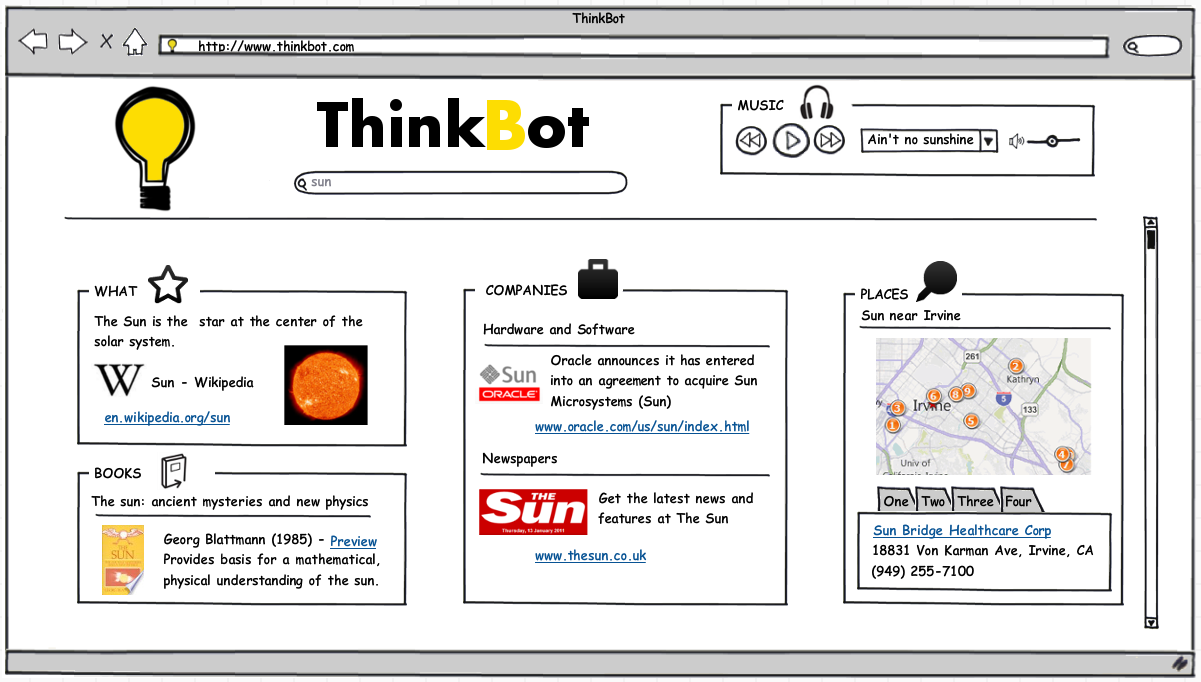
\includegraphics[width=0.9\columnwidth]{images/thinkbot.png}%
					\caption{Grouping of search results according to more general topics}%
					\label{thinkbot}%
				\end{figure}
	
	\item A less well-known search engine is \url{www.blekko.com}. Users of blekko narrow down their searches by adding so-called ``slashtags'' to their queries. A slashtag, such as \texttt{/cars} or \texttt{/law}, restricts the search result to websites of that particular topic. Besides numerous pre-defined topics, users can define and even share their own slashtags by associating websites with them. Built-in slashtags can further filter the search results. To name only a few examples, \texttt{/blog} restricts the type of a website, \texttt{/people} searches only for websites related to persons, and \texttt{/flickr} shows results from the image hosting website. Of course, multiple slashtags can be combined in one query.
	
	Example queries:
	\begin{itemize}
		\item \texttt{uci ics /people}
		\item \texttt{uci /traffic}
		\item \texttt{los angeles /baseball}
	\end{itemize}
 \end {enumerate}


\chapter{Extra Credit Questions}

\begin{enumerate}
	\item It is difficult to measure user-generated content (UGC) for several reasons. One of them is the difficulty to distinguish user-created from other content; Amazon.com, for example, consists mainly of professional content, but also includes user-generated content in form of reviews, ratings, and comments by its users.
	
	As a consequence, we limit our answer to websites that can be identified as \emph{blogs}. BlogPulse (\url{www.blogpulse.com}), a blog search engine, currently indexes 153,720,258 blogs. Technocrati (\url{www.technorati.com/state-of-the-blogosphere}), another search engine for blogs, anually publishes more elaborate statistics on ``growth and trends in the blogo\-sphere''. While there are newer reports, the report of 2007\footnote{\url{http://www.sifry.com/alerts/archives/000493.html}} is the last one to mention the number of tracked blogs: over 72,000,000. 
	
	Unfortunately, we did not find any sources that state the size of the blogo\-sphere in relation to the total size of the Web. We decided against combining other statistics on the size of the Web with the ones mentioned above, because they most likely work with different definitions and methods of counting.
\end{enumerate}



\chapter{Programming Questions}

\begin{enumerate}
	\item	\begin{enumerate}
					\item \todo{Describe complexity of palindrome algorithm}
					\item In order to find the longest lipogram in a given text file, our algorithm scans the text only once. Each character is regarded separately: \begin{itemize}
							\item If a valid character, i.e. a letter of the English alphabet but not \texttt{e} or \texttt{E}, is detected, it is added to the current lipogram.
							\item If an invalid character, i.e. a non-ASCII symbol, is detected, it is added to the current lipogram and the counter for invalid characters increases.
							\item If either \texttt{e} or \texttt{E} is detected, the lipogram is compared to the currently longest lipogram(s). If it is equally long or even longer and it consists of less then 30\% invalid characters, it is added to the list of longest lipograms. If it is longer, the smaller ones are discarded.
						\end{itemize}
						Since the algorithm runs only once through the text file and examines each detected character only once, the runtime complexity of our algorithm is $O(n)$.
				\end{enumerate}
\end{enumerate}


%\pagebreak
%\begin{thebibliography}{XXX}
%	\bibitem{1} {\it Watever}
%\end{thebibliography}



\end{document}
